\documentclass[a4paper,12pt]{article}
\usepackage[ukrainian,english]{babel}
\usepackage{ucs}
\usepackage[utf8]{inputenc}
\usepackage[T2A]{fontenc}
\usepackage{amsmath}
\usepackage{amsfonts}
\usepackage{graphicx}
\begin{document}
	Бекешева Анастасія ФІ-12\\
	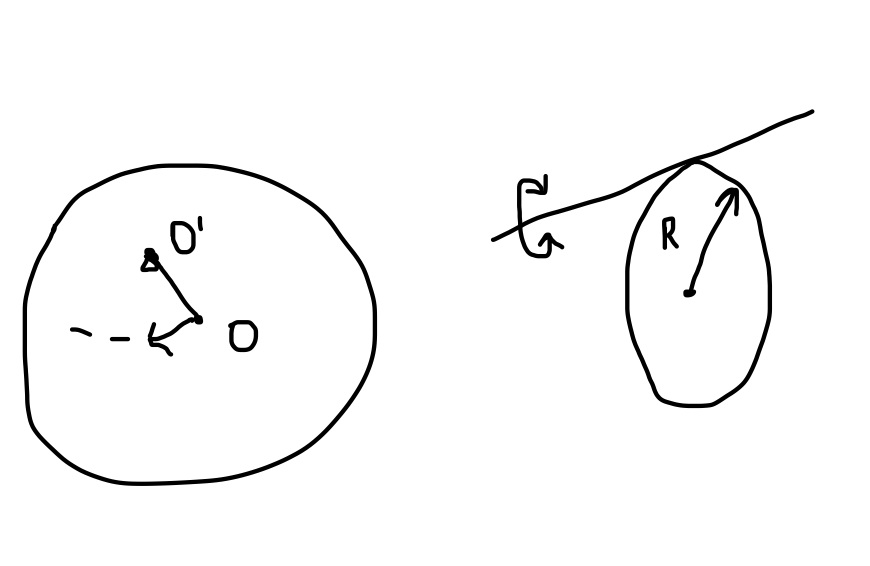
\includegraphics[width=5cm]{graph9}\\
	Періаод: $T=2\pi\sqrt{\frac{J}{mgx}},\>x=\frac R2$(по умові), $T=2\pi\sqrt{\frac{2J}{mgR}}$\\Момент інерції диска: $J=J_0+\frac {mR^2}4=\frac {mR^2}2+\frac {mR^2}4=\frac34mR^2\\\Rightarrow T=2\pi\sqrt{\frac{2\cdot\frac34mR^2}{mgR}}=2\pi\sqrt{\frac{3R}{2g}}$\\Частота: $\nu=\frac1T=\frac1{2\pi}\sqrt{\frac{2g}{3R}}\\$ Зведена довжина: $L_\textrm{зв}=\frac{T^2g}{4\pi}=\frac{4\pi 3Rg}{2g4\pi}=\frac32R$ 
\end{document}
